\documentclass[aspectratio=169]{beamer}
\setbeamertemplate{navigation symbols}{}
\usepackage{color,amsmath,comment, subfigure}
\usepackage{booktabs}
\usepackage{url}

\def\imagetop#1{\vtop{\null\hbox{#1}}} %http://tex.stackexchange.com/questions/23521/tabular-vertical-alignment-to-top

%\setbeameroption{show notes}

%%%%%%%%%%%%%%%%%%%%%%%%%%
\title[]{Class 16: Experimental studies of contagion}
\author[]{Matthew J. Salganik}
\institute{Sociology 204: Social Networks\\Princeton University}
\date[]{
2/3 Is voting contagious?
\vfill

\begin{flushleft}
\vspace{0.6in}

\includegraphics[width=0.1\textwidth]{figures/cc.png}
\end{flushleft}
}

%%%%%%%%%%%%%%%%%%%%%%%%%%%
% SWBAT Describe the challenge of isolating contagion from other causes of similarity
% SWBAT Describe different designs to measure social contagion
% SWBAT Use ideas of internal validity and external validity to identify concerns with experiments
% SWBAT TODO
%%%%%%%%%%%%%%%%%%%%%%%%%%%%%%%%%%%%%%%%%%
\begin{document}
\frame{\titlepage}
%%%%%%%%%%%%%%%%%%%%%%%%%%%
\begin{frame}

\begin{center}
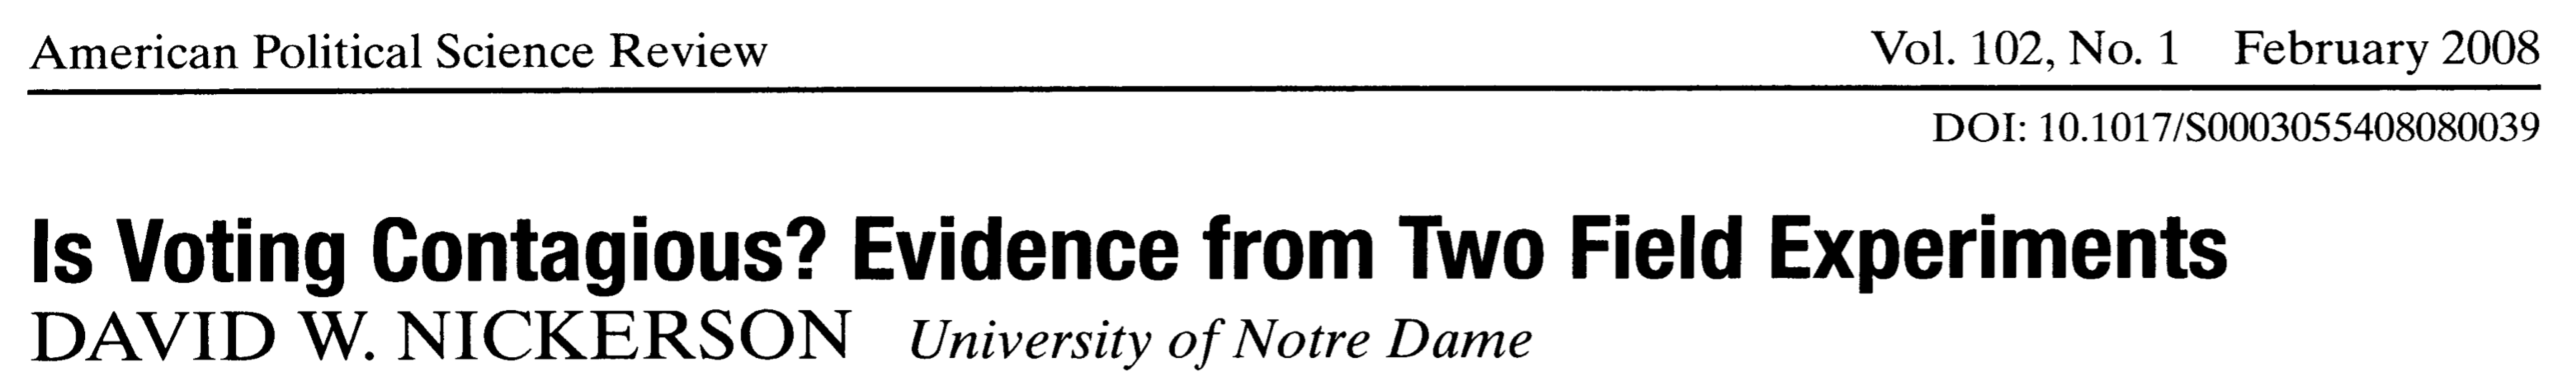
\includegraphics[width=\textwidth]{figures/nickerson_voting_2008_title}
\end{center}

\vfill
\url{http://doi.org/10.1017/S0003055408080039}

\end{frame}
%%%%%%%%%%%%%%%%%%%
\begin{frame}

\begin{center}

\includegraphics[width=0.5\textwidth]{figures/point}
\end{center}

\end{frame}
%%%%%%%%%%%%%%%%%%%%
\begin{frame}

\begin{center}
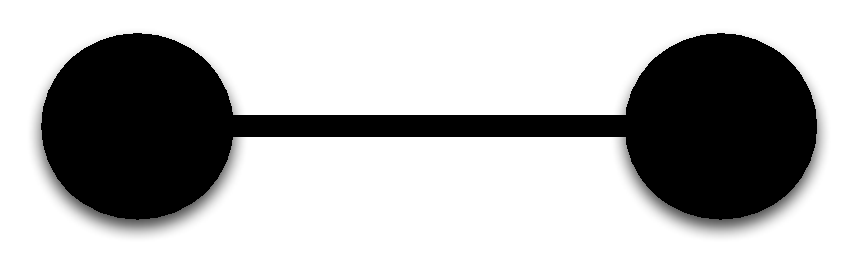
\includegraphics[width=0.8\textwidth]{figures/dyad}
\end{center}

\end{frame}
%%%%%%%%%%%%%%%%%%%
\begin{frame}

\begin{center}

\includegraphics[width=0.9\textwidth]{figures/nickerson_schema}
\end{center}

Contagion effect: $\alpha = \frac{S}{T}$

\vfill
Note that there is nothing specific in this design to voting.  This could be any intervention.

\end{frame}
%%%%%%%%%%%%%%%%%%%%
\begin{frame}

\begin{center}
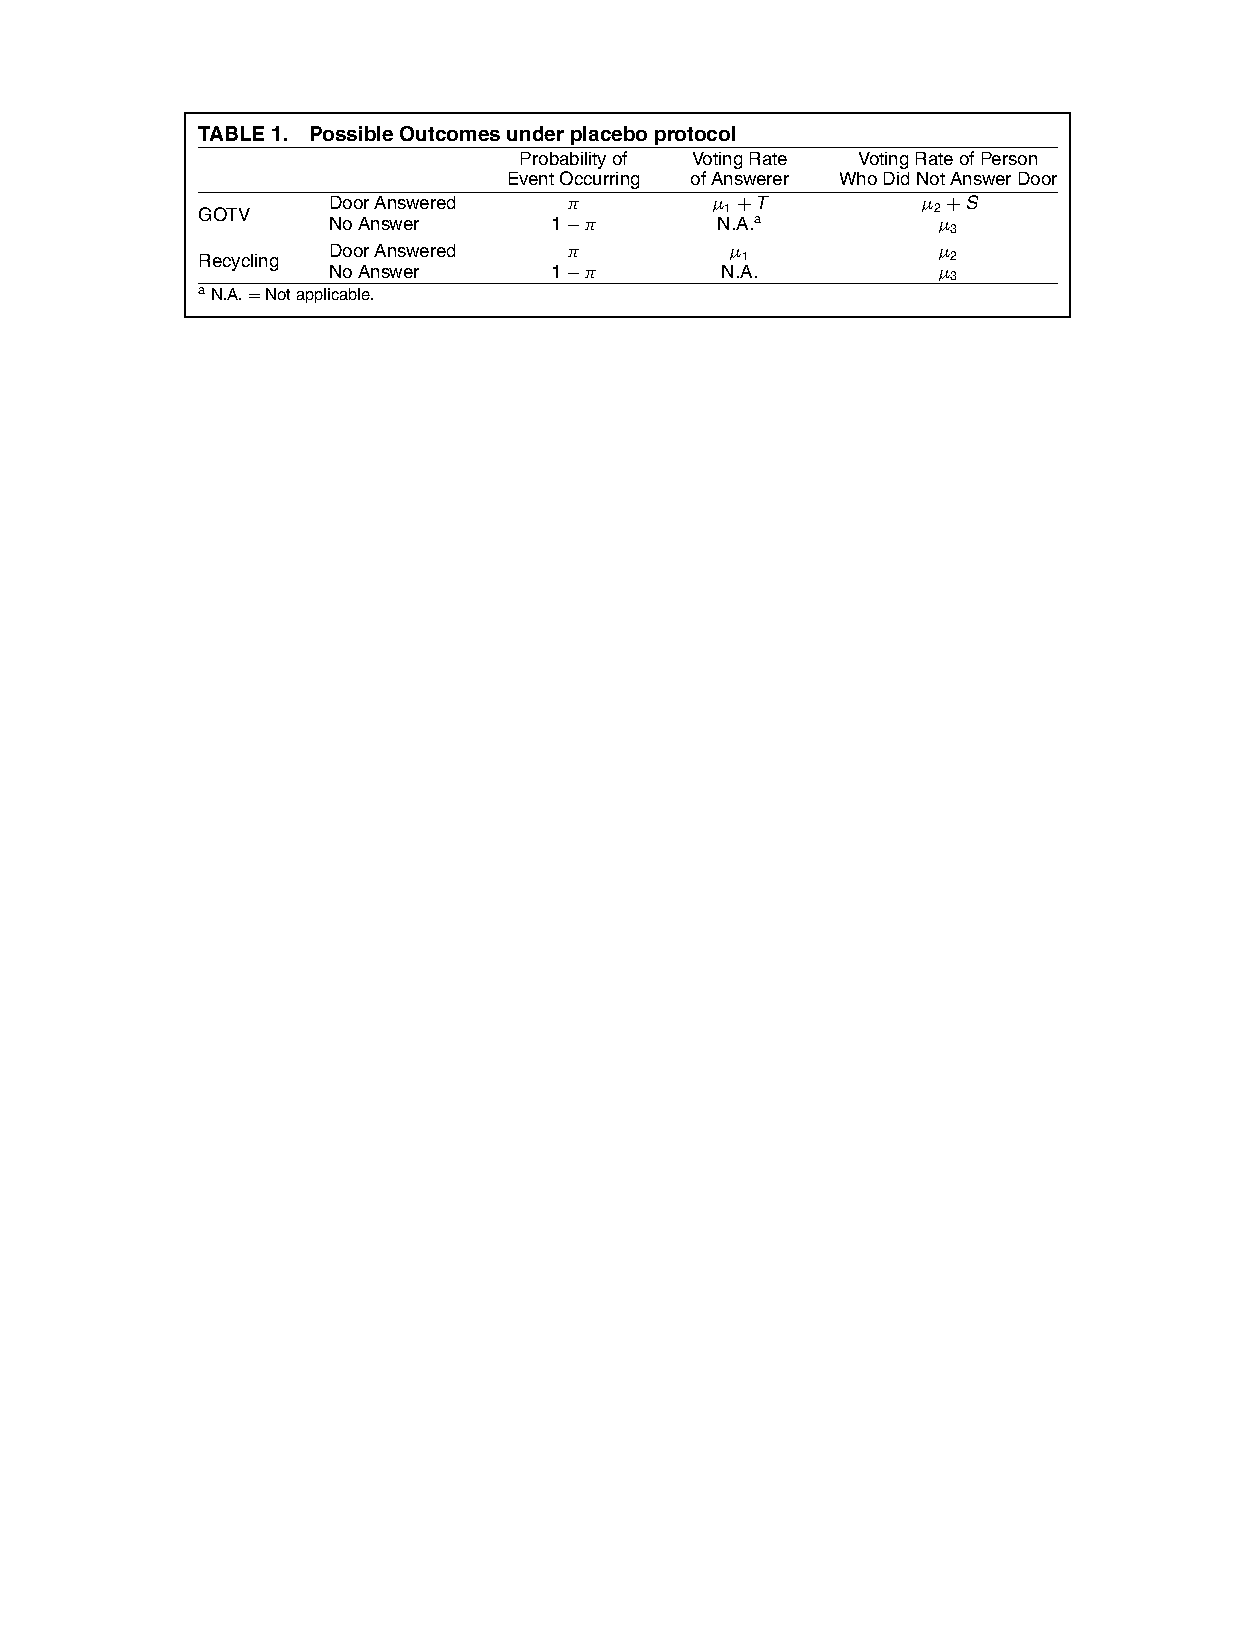
\includegraphics[width=1\textwidth]{figures/nickerson_voting_2008_tab1}
\end{center}

\vfill

The role of the recycling intervention is to create a ``fair'' comparison.
\end{frame}
%%%%%%%%%%%%%%%%%%%%%%%%
\begin{frame}

\begin{center}
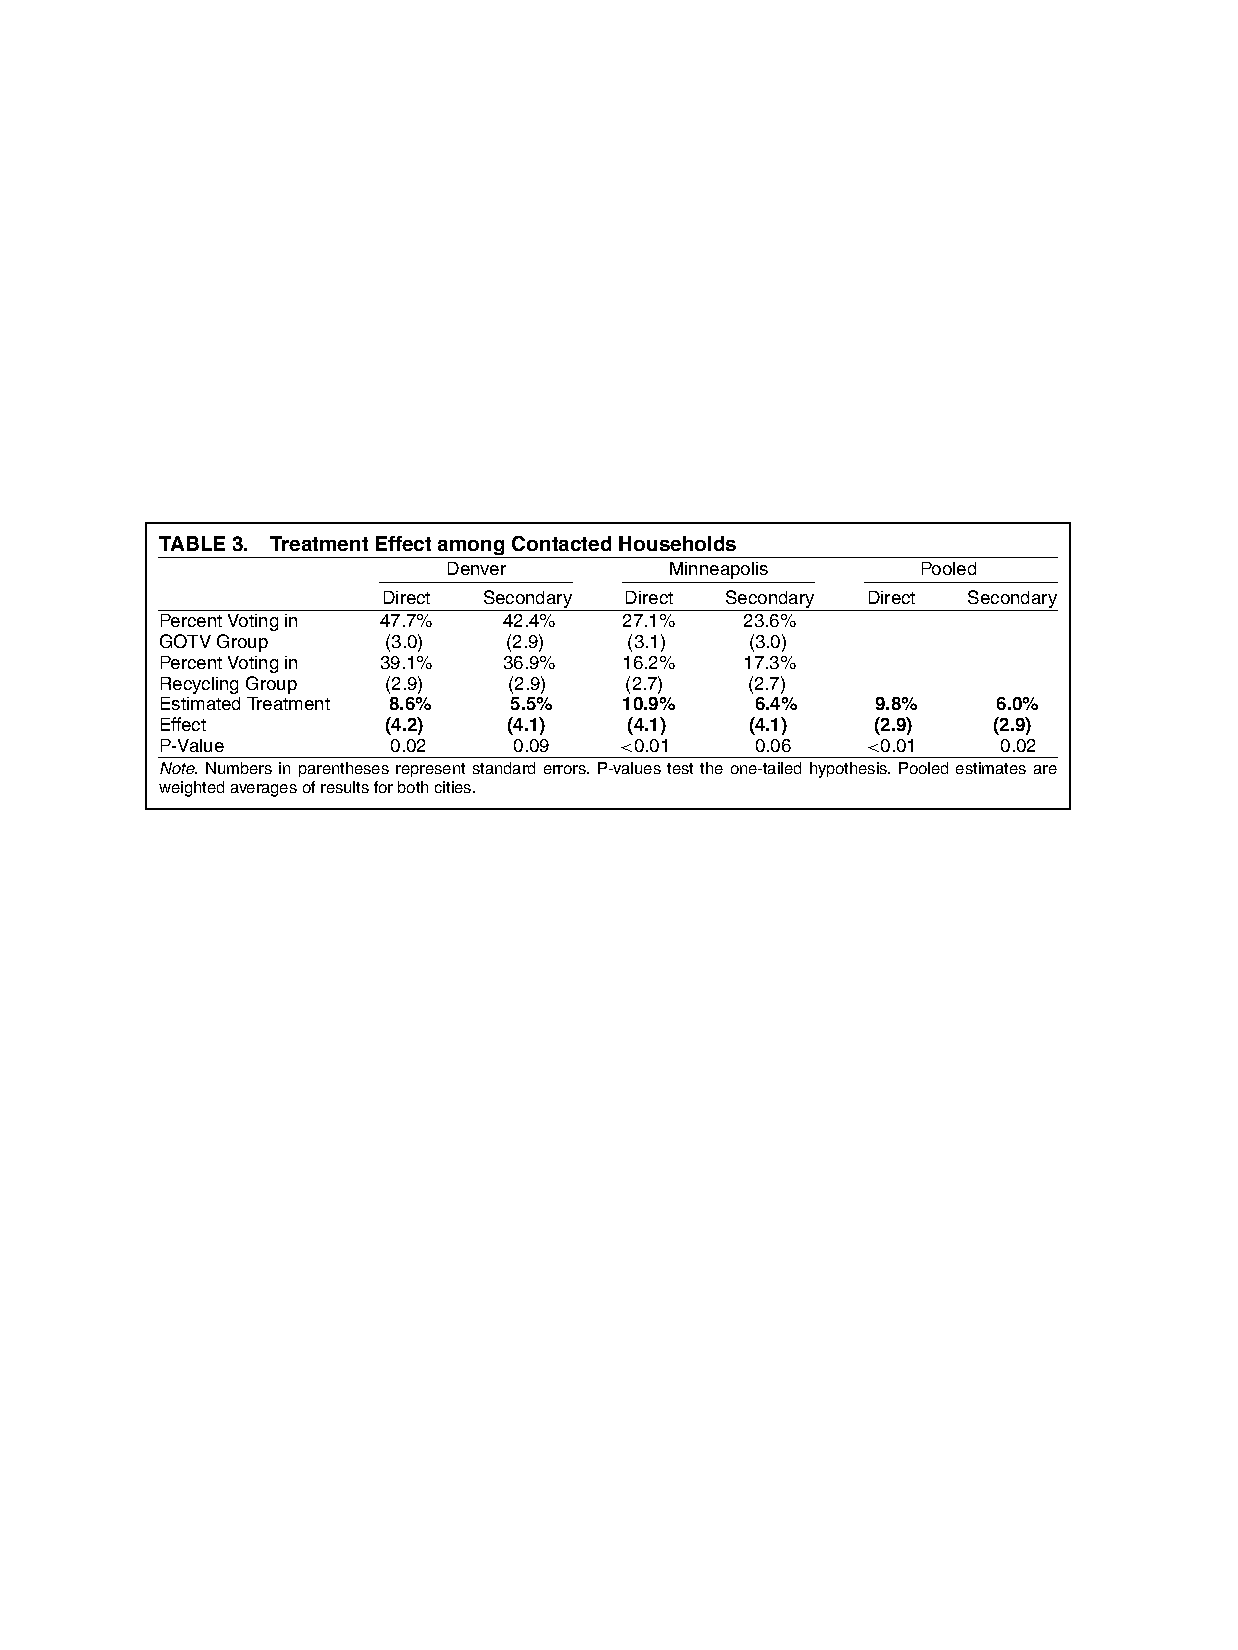
\includegraphics[width=1\textwidth]{figures/nickerson_voting_2008_tab3}
\end{center}

\end{frame}
%%%%%%%%%%%%%%%%%%%%%%%%%
\begin{frame}

How much should you trust these results? Internal and external validity

\end{frame}
%%%%%%%%%%%%%%%%%%%%%%%%%
\begin{frame}

\begin{center}
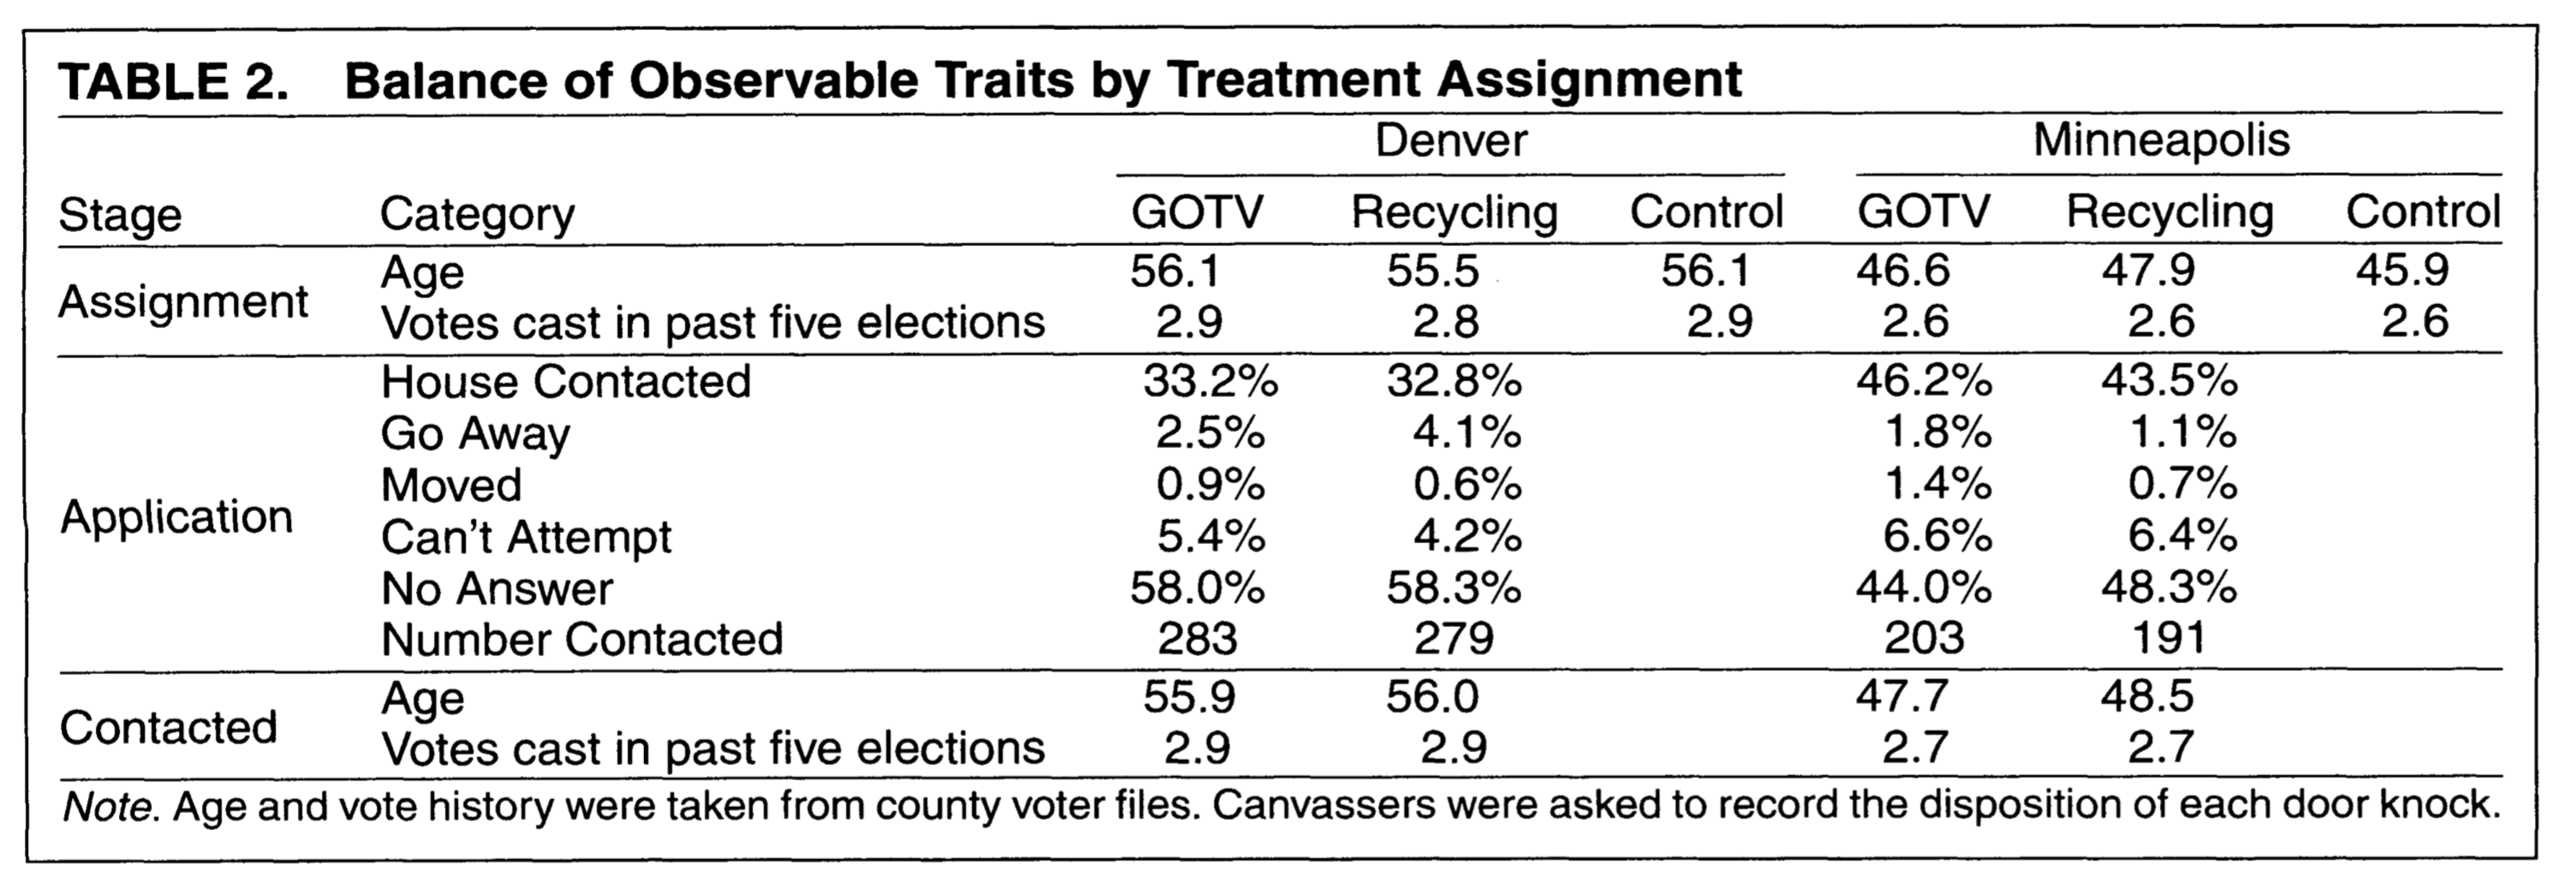
\includegraphics[width=1\textwidth]{figures/nickerson_voting_2008_tab2}
\end{center}

Internal validity: it looks like the get-out-the-vote people and the recycling people are similar

\note{
Groups looks similar, it is a bit surprising that no statistical test here
}

\end{frame}
%%%%%%%%%%%%%%%%%%%%%%%%%
\begin{frame}

External validity (partial list)
\begin{itemize}
\item ties within households are different from other ties \pause
\item households in this study might be different from other households \pause
\item these results are from a low salience election (might be different in a presidential election) \pause
\item other behaviors might not be as contagious as voter turnout
\end{itemize}

\end{frame}
%%%%%%%%%%%%%%%%%%%%%%%%%
\begin{frame}

Notes on application:
\pause
\begin{itemize}
\item Need to count the spillover (if you generate 100 direct votes, you also generate about 60 indirect votes)
\pause
\item No idea about mechanism so hard to design more contagious treatments
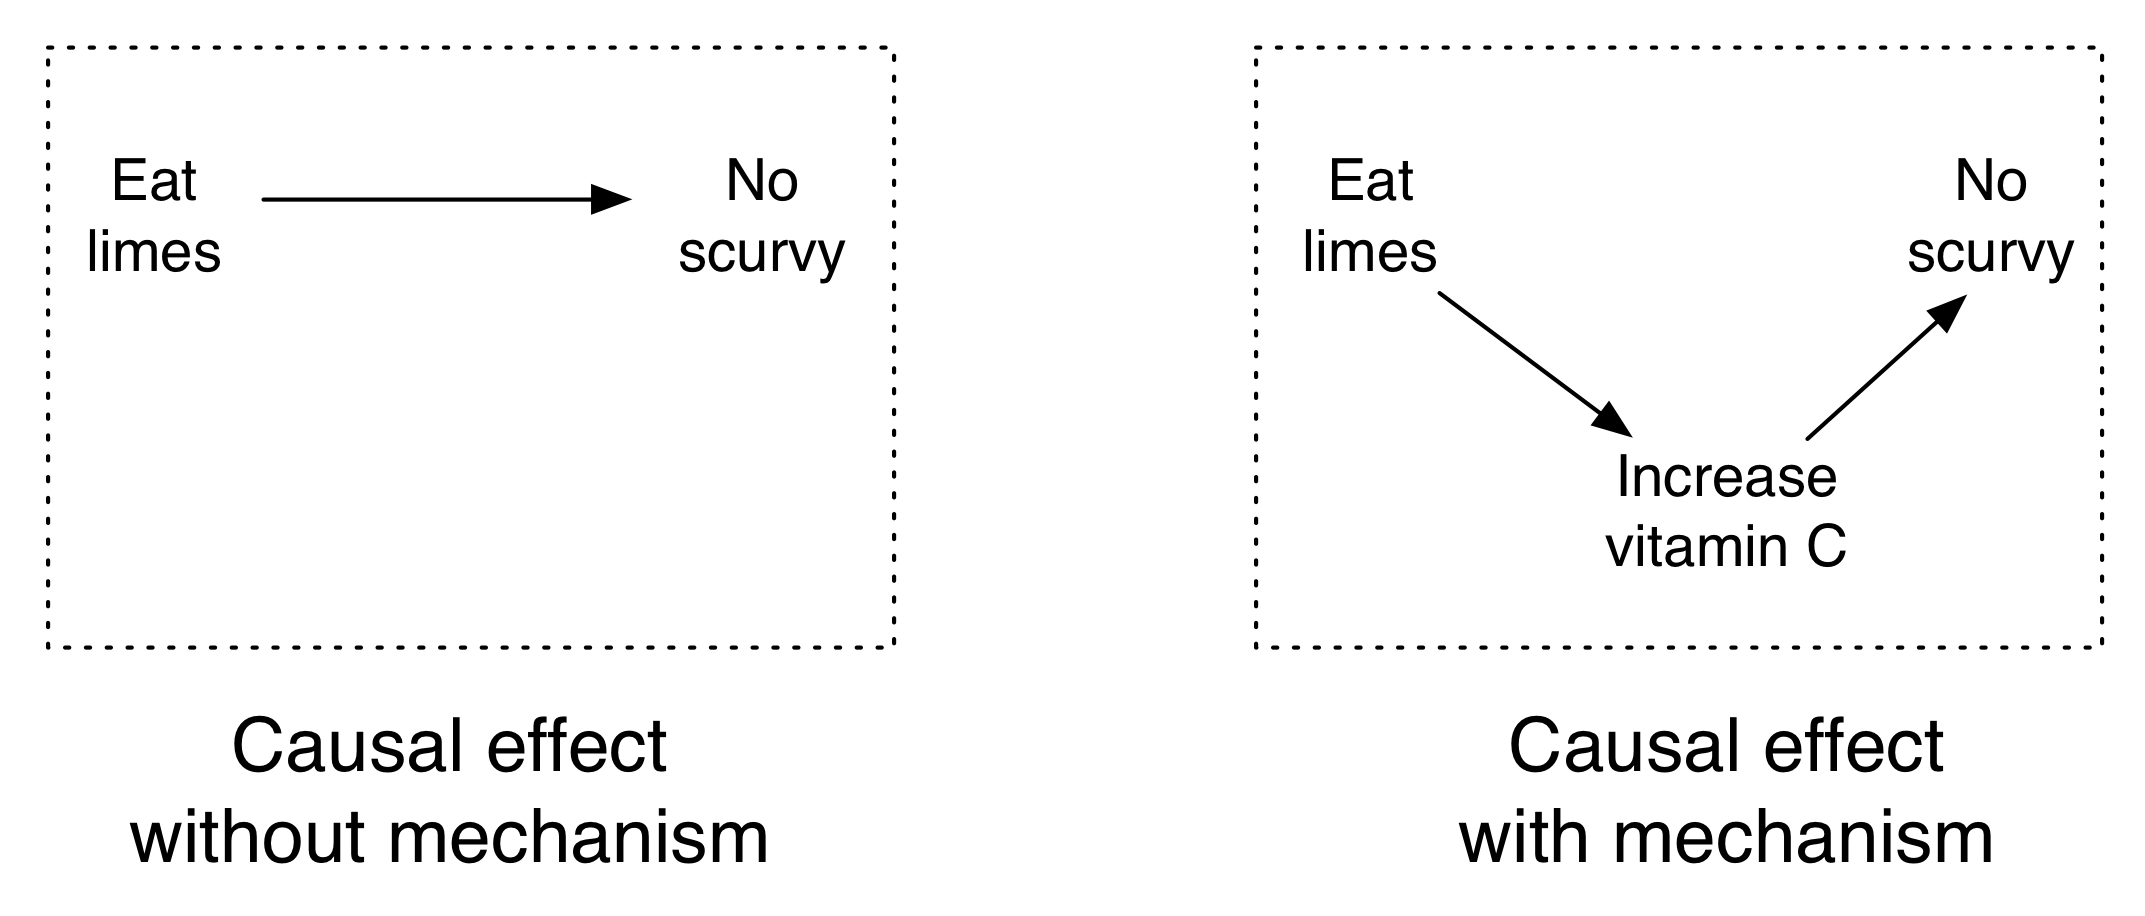
\includegraphics[width=0.9\textwidth]{figures/bitbybit4-10_mechanism_schematic}
\end{itemize}

\end{frame}
%%%%%%%%%%%%%%%%%%%%
\begin{frame}

\begin{center}
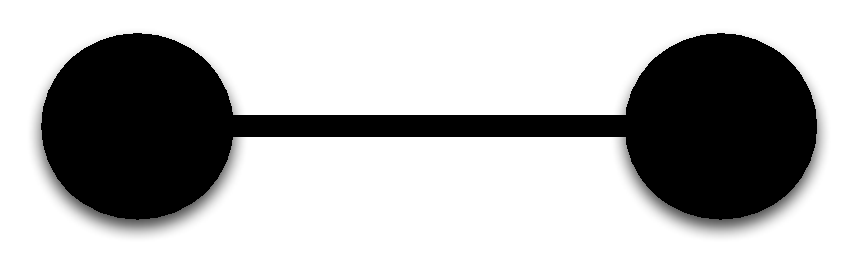
\includegraphics[width=0.8\textwidth]{figures/dyad}
\end{center}

\begin{itemize}
\item contagion of voting via ``intervene and spillover'' design \pause
\item contagion of emotion via an ``edge-control'' design
\end{itemize}

\end{frame}

\end{document}
